\chapter{Related Works}
\label{chapter:related-works}
\thispagestyle{empty}
\section{Watermark Overview}
Watermarking involves modifying a piece of content to include a message related to that content. The origins of watermarking can be traced back to medieval times, evolving alongside advancements in papermaking and the growing need for document authentication and security. The practice first emerged in 13th century Italy, where papermakers integrated basic designs or symbols into paper molds, resulting in subtle variations in thickness. When held up to light, these watermarks became visible, functioning as identification for the papermaker or as an indicator of quality. Watermarking involves modifying a piece of content to include a message related to that content. The origins of watermarking can be traced back to medieval times, evolving alongside advancements in papermaking and the growing need for document authentication and security. The practice first emerged in 13th century Italy, where papermakers integrated basic designs or symbols into paper molds, resulting in subtle variations in thickness. When held up to light, these watermarks became visible, functioning as identification for the papermaker or as an indicator of quality.

By the 18th century, watermarks began incorporating more elaborate designs and patterns, often reflecting the brand of the paper manufacturer or adding an artistic touch. This period marked a shift from purely utilitarian watermarks to those with aesthetic appeal. In the early 20th century, the advent of digital technology led to the transformation of traditional paper watermarks into digital counterparts. In the realm of digital media, these digital watermarks serve diverse purposes, including safeguarding copyright, authenticating content, and facilitating tracking. They are imperceptible to the human eye and became prevalent in the late 20th century, embedded within digital files such as images or documents. Nowadays, watermarks continue to fulfill essential roles in security, branding, and authentication across physical and digital domains, adapting to the evolving needs of industries and technologies.

Paper watermarks first appeared in Italy in 1282, over a thousand year since papermaking had been invented in China. The marks were made by adding thin wire patterns to the paper molds. The earliest watermarks were used for practical functions such as identifying the molds on which sheets of papers were made, or as trademarks for ownership, or they might just represent mystical signs or serve as decoration. By the eighteenth century, they have been used in Europe and America for precise purposes, trademarks and manufacturing records. It was also the first time watermarks were used as anticounterfeiting measures on money and other documents. From that time, watermark embedding systems and watermark attacking systems prompted advances for each other, as a subbranch of security and steganography.

\subsection{Watermark Embedding}
In general, watermarks can be as simple as an extra logotype or text added to an image that are subtle with human visual system, or an imperceptible signal embedded to an original signal. Subsequently, watermarks can be broadly classified into two primary categories - visible and invisible.

Visible watermarks are intentionally noticeable and easily seen by the human eye. Typically overlaid onto the surface of an image or document, they often consist of logos, text, or symbols. The principal aim of visible watermarks is to identify the origin or ownership of the content and deter unauthorized use. While effective in conveying ownership, visible watermarks may occasionally impact the aesthetic appeal of the content.

On the other hand, invisible watermarks are like secret codes you cannot see right away. They get mixed into the picture using digital tricks, such as adding noise or embedding unique code within the pixels of a digital image without changing how it looks. Invisible watermarks do different jobs, like protecting copyrights, proving if something is real, or keeping track of things. They are useful for digital stuff, like pictures or documents, because you do not see any changes on the outside. To find invisible watermarks, you need special computer programs or smart processes that can uncover the hidden information.

In our project, we are focusing on those watermarks that catch your eye—the visible ones. They mess with the image when they are added, and that is the puzzle we are tackling. We are figuring out how to use a diffusion-based method to bring back the original image after we have wiped out those noticeable watermarks, like totally removing them from the picture.

We now then work on putting the watermark into images. The aim is to enhance the image's privacy, adding an extra layer of security. The introduction of a watermark provides a level of protection for the image. Watermarks come in various types, such as those made of text or images. In our project, we are specifically concentrating on image watermarks. Our objective is to embed the image watermark into the original image, making it challenging to identify or detect compared to text watermarks, which are somewhat easier to recognize. Subsequently, we plan to examine and remove these watermarks through detection methods.

There are various methods to incorporate a watermark into an image. Tao et al. \cite{tao2014robust} have researched some methods to embed a robust watermark, ranging from random embedding to intentional placement. In intentional embedding, the watermark can alter the image's appearance, making it challenging for humans to observe or confusing for classifier models, leading to incorrect predictions. In our approach, we choose to randomly embed the watermark within the image, in which details will be discussed in Chapter \ref{chap:experiment}. This section will delve into the specifics of our method for watermark embedding.


In general, watermarks can be as simple as an extra logotype or text added to an image that are subtle with human visual system, or an imperceptible signal embedded to an original signal. Those in the former case are conventionally called visible watermarks, where diffusion models can be applied to transform a watermarked region or the whole image into a realistic unwatermarked version. Those in the latter case are called invisible watermarks with two broad groups of generating models - \textit{communication-based} models and \textit{geometric models} \cite{cox2007digital}. We focus on visible watermarks only. A visible watermark embedding algorithm should satisfy some requirements, such as

\begin{enumerate}
    \item The watermark is perceptible in both gray and colored images.
    \item The watermark should be perceptible in pixels with different characteristics: texture, plain and edge.
    \item The watermark should not be too obtrusive.
    \item The watermark should be robust against several common attacks.
    \item Watermark embedding process should be automatic for kinds of images.
\end{enumerate}

An image can be represented a three-channel two-dimensional array. Compressed into the gray scale, each pixel takes integer values in the interval $[0,256]$.  The following watermark embedding model for binary watermark \cite{yu2013new} is based on the observation that the ability of human eyes to distinguish between two close pixel values tend to be highest in the interval $[64,128]$, i.e. for a pixel $p\in [64,128]$, a human may be able to distinguish between $p$ and $p+1$. Denote by $y$ this minimal perceptible difference. They approximate the relation as
\begin{equation}
    y=\begin{cases}
        -\dfrac{1}{8}p+6,             & \text{ if } p\in [0, 32]   \\
        -\dfrac{1}{32}p+3,            & \text{ if } p\in [33, 64]  \\
        -\dfrac{1}{96}p+\dfrac{1}{3}, & \text{ if } p\in [65, 255] \\
    \end{cases}
\end{equation}

\begin{figure}
    \centering
    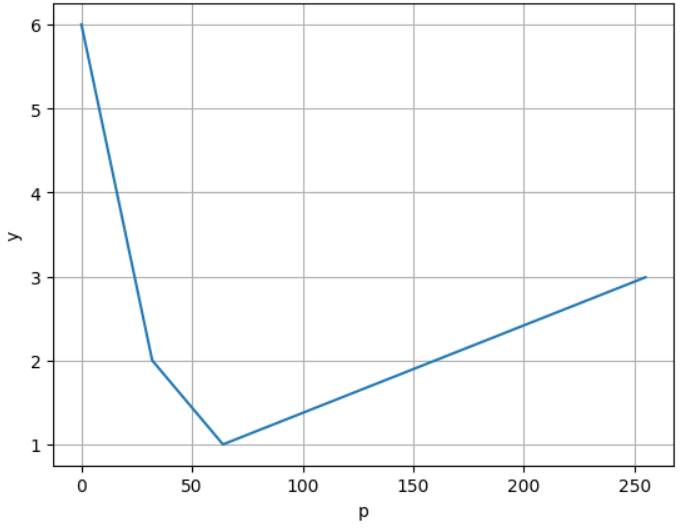
\includegraphics[width=0.5\linewidth]{img/resolution.png}
    \vspace{0.5cm}
    \caption{The approximation of human eye resolution on the gray scale}
    \label{figure:human-eye-resolution}
\end{figure}

Therefore, the difference between a clean pixel and a watermarked pixel must obey this human distinguishing ability. The watermark strength $\alpha$ depending on the pixel value is given by
\begin{equation}
    \alpha(p)=cy(p),
\end{equation}
where $c$ is a constant hyperparameter. The watermarked image is obtained pixel-by-pixel by
\begin{equation}
    p'(i,j)=p(i,j)+\alpha
    (p(i,j))w(i,j),
\end{equation}
where
\begin{itemize}
    \item $p(i,j)$ is the original pixel
    \item $w(i,j)\in\{0,1\}$ is the watermark value
\end{itemize}

The embedding process is applied for each channel and finally combined to a single watermarked image.

\subsection{Watermark Removal}
% intro with surveys
Digital watermarks are frequently employed for copyright identification in images, preventing unauthorized use of online images. Additionally, techniques for attacking watermarks aim to effectively eliminate watermarks from host images. The strength of a watermark against such attacks is crucial for safeguarding image copyrights. Methods for removing watermarks have been investigated to assess and enhance the durability of watermarks. In this section, we will explore existing methods and discuss our approach to watermark removal.

Oldest methods for getting rid of watermarks usually require users to point out where the watermark is located, and then they use special features to remove it, such as Independent Component Analysis \cite{pei2006novel} or Color Space Transformation \cite{park2012identigram}. Also, some methods make use of multiple images \cite{dekel2017effectiveness} \cite{gandelsman2019double}. But, these methods need a lot of information ahead of time, and they only work well on a limited number of examples.

\begin{figure}[H]
    \centering
    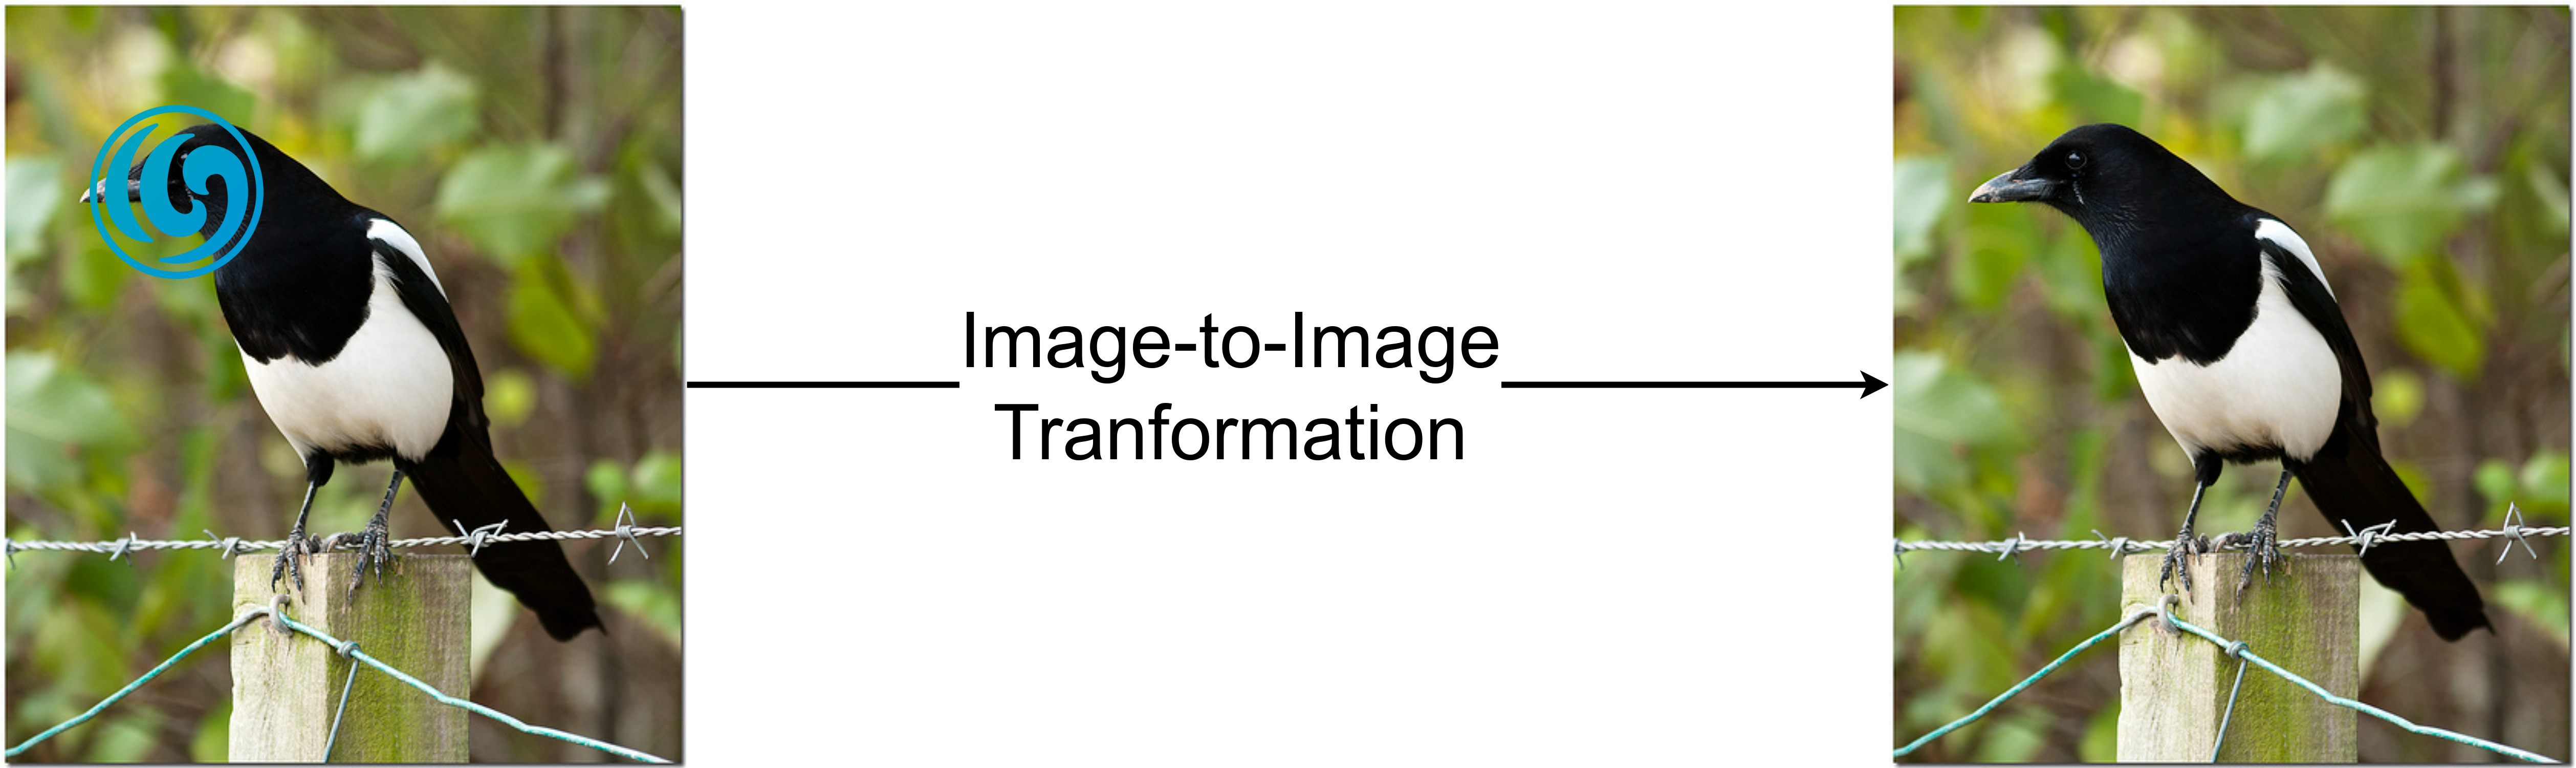
\includegraphics[width=0.75\linewidth]{img/watermark_removal_1.png}
    \caption{Watermark Removal with Image-to-Image methods}
    \label{figure:img2img1}
\end{figure}

More recently, deep learning-based methods show great power in many computer vision tasks \cite{he2016deep}, and this approach has been applied to remove visible watermarks too \cite{li2019towards} \cite{cheng2018large}  \cite{hertz2019blind}. But, before using these methods, you need a detection model that can already identify watermarks \cite{cheng2018large}, or they only focus on getting rid of the watermark without thinking about the whole image as an Image-to-Image Translation problem \cite{li2019towards}, as generally illustrated in Figure \ref{figure:img2img1}. Plus, the datasets they often use only have gray-scale watermarks. Nowadays, though, most watermarks are in color. Recently, a method was designed to find, erase, and fix the motif in just one go \cite{hertz2019blind}. However, these methods do not pay much attention to learning about the damaged part of the image.

% \textcolor{red}{CNN version (U-Net): https://arxiv.org/pdf/2403.05807.pdf}
% \textcolor{red}{Note about one-stage watermark removal}
% \subsection{Image-to-Image methods}
% Summary some methods in Image-to-Image


\section{Two-stage Watermark Removal}

The mentioned methods in the previous section mainly focus on transforming a watermarked image to an unwatermarked one, which we can think of as one-stage watermark removal. In this section, we discuss models relevant to our approach, including segmentation models (SegFormer and SAM) and a diffusion-based inpainting model (I$^2$SB). These models build up our two-stage watermark removal pipeline, which is discussed in details in Chapter \ref{chap:experiment}.

Before Transformer (see Section \ref{section:transformer}), U-Net \cite{ronneberger2015u} was popular for semantic segmentation task. Segmentation Transformer (SETR) \cite{zheng2021rethinking} was one of early applications of Transformer for semantic segmentation, achieving considerable improvement over CNNs. SegFormer \cite{xie2021segformer} was developed in motivation of this work, with Efficient Self-attention. Recently, Segment Anything Model (SAM) \cite{kirillov2023segment} was designed for the ability to run on low-end devices. In this section, we discuss two latest models, SegFormer and SAM, which are also those used in our watermark segmentation phase.

\subsection{SegFormer}
\label{intro:segformer}
SegFormer made use of multi-head attention mechanism, but highly specialized for semantic segmentation task.

\begin{figure}[ht]
  \centering
  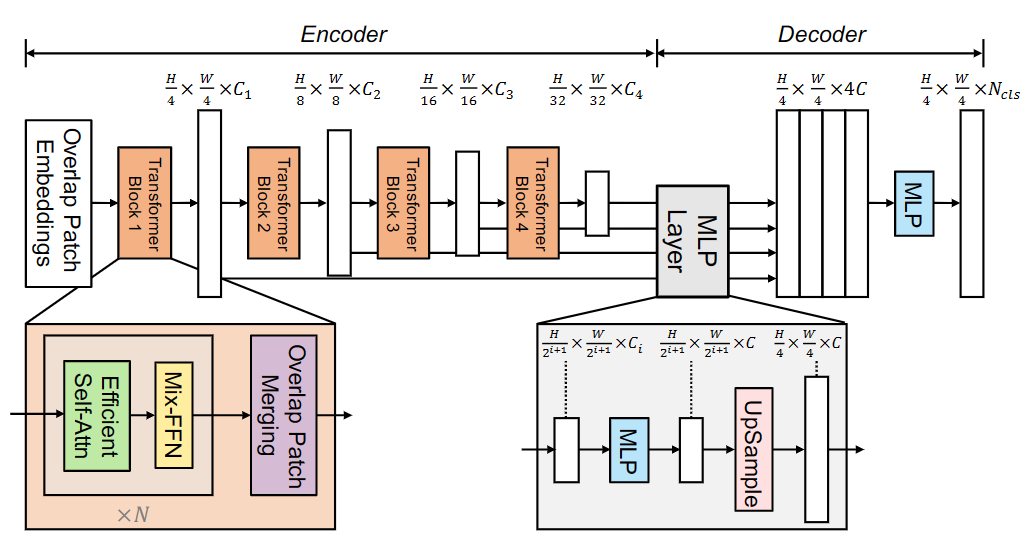
\includegraphics[width=0.7\linewidth]{img/segformer.png}
  \vspace{0.5cm}
  \caption{SegFormer Architecture}
  \label{figure:segFormer-architecture}
\end{figure}

As can be seen in Figure \ref{figure:segFormer-architecture}, there are two major components in the architecture, namely the Overlap Patch Embedding, Transformer Block and the MLP Layer, whose details are delved into in following sections.

\subsubsection{Encoder}

\textbf{Overlap Patch Embedding.} Originally in Vision Transformer (ViT) \cite{dosovitskiy2020image}, an image of size $H\times W\times 3$ is divided into $\frac{HW}{P^2}$ patches of size $P\times P \times 3$. Each patch is then flattened and linearly projected in to a $C$-dimensional vector, where $C>3$, returning a sequence of size $\frac{HW}{P^2}\times C$. The patches in this case have no overlaps.

SegFormer employed Overlap Patch Embedding, with two additional hyperparameters $s$ and $p$ for stride and padding, similarly to CNNs. In particular, the authors of SegFormer used $(P,s,p)\in\{(7,4,3), (3,2,1)\}$, result in a sequence size $\frac{HW}{4} \times C$, while preserved the local continuity around those patches.

\textbf{Efficient Self-Attention.} This is an subblock of the Transformer block. After extracted as the keys $\mathbf{K}$ and queries $\mathbf{Q}$ of the same size as the sequence, the matrices go through a self-reduction process of ratio $r$. For instance, let $N=\frac{HW}{4}$, we have
\begin{align*}
  \mathbf{K'} & = \mathrm{Reshape}\left(\dfrac{N}{r}, C\cdot r\right)(\mathbf{K}) \\
  \mathbf{K}  & = \mathrm{Linear}\left(\dfrac{N}{r}, C\right)(\mathbf{K'}).
\end{align*}
Thus, $\mathbf{K}$ is reduced to dimension $\frac{N}{r}\times C$ and similarly for $\mathbf{Q}$. The complexity is reduced from $O(N^2)$ to $O\left(\frac{N^2}{r}\right)$ comparing to original Multi-head Attention \cite{xie2021segformer}. In particular, the matrices $\mathbf{K}$, $\mathbf{Q}$ and $\mathbf{V}$ are constrained to be of equal size, enabling them to be generated simultaneously from the token sequence, which results in improved computational performance.

\textbf{Mix-FFN.} This subblock is used as an alternative to Positional Encoding in ViT that only takes care of the distance between the tokens. The approach in ViT leads to the drop of accuracy for semantic segmentation task when the test set resolution differs from the training set. In SegFormer, the authors included a convolutional layer to encode positional information
$$\xbf_{\mathrm{out}} = \mathrm{MLP}(\mathrm{GELU}(\mathrm{Conv_{3\times 3}(\mathrm{MLP}(\xbf_{in}))})).$$
Their approach was based on an argument that adding PE to feature map is not necessary in semantic segmentation, and was empirically proved to be sufficient for this task.


\textbf{Overlapped Patch Merging.} This is the final subblock of the Transformer block that reshapes the previous output to size $\frac{W}{2}\times \frac{H}{2} \times C$, and processes similarly to Overlap Patch Embedding, returning a sequence of size $\frac{WR}{16}\times C_1$, where $C_1>C$. The other three following Transformer Blocks work similar, getting the sequence after the previous block and outputting a sequence of size $\frac{WR}{2^{2i+2}}\times C_i$, for $i\in\{2,3,4\}$.

\subsubsection{Decoder}
After each Transformer Block, the sequence is reshaped to get hierarchical representation of size $\frac{W}{2^{i+1}}\times \frac{H}{2^{i+1}}\times C_i$, for $i\in{1,2,3,4}$. Each representation goes through an MLP and then is unsampled to size $\frac{W}{4}\times \frac{H}{4}\times 3$. The representations are concatenated to $\frac{W}{4}\times \frac{H}{4}\times 12$. The last MLP (the blue block in Figure \ref{figure:segFormer-architecture}) gives the output $\frac{W}{4}\times \frac{H}{4}\times N_{\mathrm{cls}}$, where $N_{\mathrm{cls}}$ is the number of classes. Intersection over Union (mIoU) was selected to be the loss function.

\subsection{Segment Anything}
\label{sec:intro-sam}
The other choice for the watermark detection stage in our pipeline is the Segment Anything model (SAM) developed by Meta \cite{kirillov2023segment}, a considerable revolution in semantic segmentation task, as it allows prompts from user. The design is claimed to be optimized to work in real-time. The model consists of an image encoder, a prompt encoder and a lightweight mask decoder. We will delve into the details as follows.

\begin{figure}
  \centering
  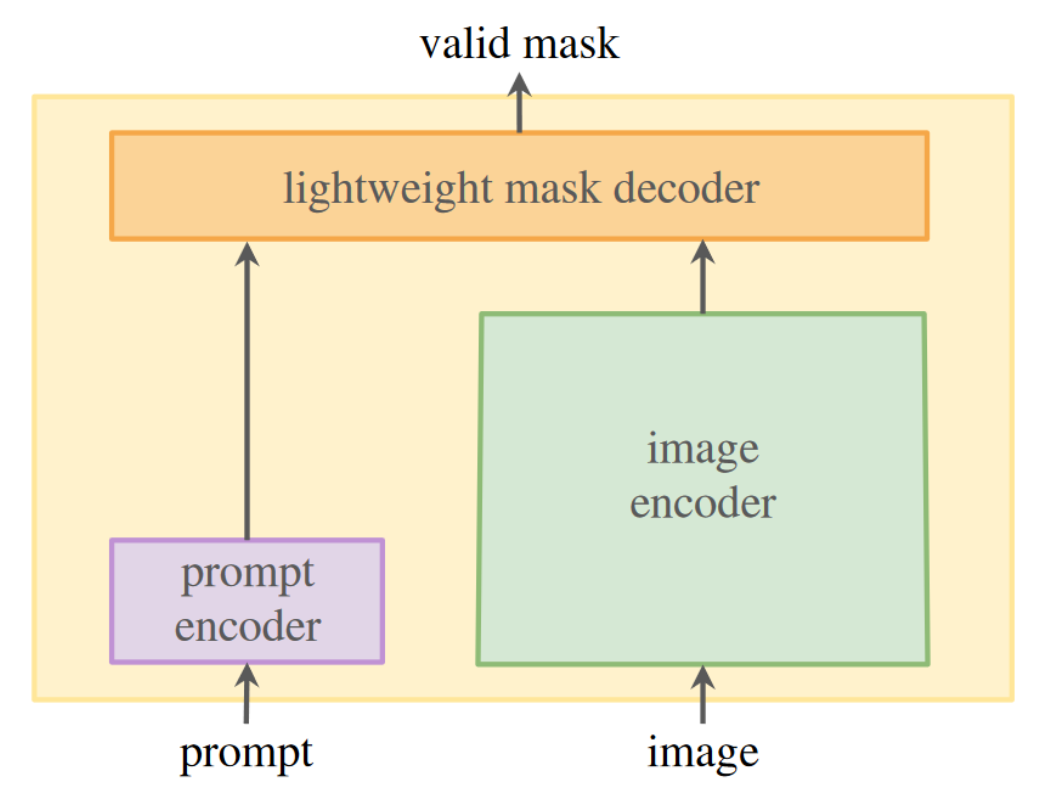
\includegraphics[width=0.6\textwidth]{img/segment-anything-model.png}
  \vspace{0.25cm}
  \caption[The overall architecture of Segment Anything model]{The overall architecture of Segment Anything model \cite{kirillov2023segment}}
\end{figure}

\subsubsection{Image Encoder}
The authors of the Segment Anything model followed standard practices, that they firstly rescale an image and pad the shorter side to attain an input resolution of $1024\times1024$. They employed several ViT backbones \cite{dosovitskiy2020image}, one of them is a ViT-H/16, followed by a Masked Autoencoder \cite{he2022masked}, returning an image of 16-time lower resolution. The image is then passed through convolutional layers to arrive at an output size of $256\times 64\times 64$.

\subsubsection{Prompt Encoder}
The model allows prompts of two types: sparse (points, boxes, text) and dense (masks). Each prompt is mapped to a $256$-dimensional vectorial embedding. A point is represented by the sum of a foreground-background learned embedding and a positional encoding. The latter value is a general approach of the sinusoid function called Fourier features \cite{tancik2020fourier}. A box is represented by an representation pair. For the top-left corner, the representation is the sum its positional encoding and its learned ``top-left corner'' embedding. A similar structure is applied for the bottom-right corner, except for that a learned ``bottom-right corner'' embedder is used. A text encoder can be any available one. The authors used continuous bag of words and Text Transformer \cite{vaswani2017attention} for their experiments. A mask is firstly converted a 4-time lower resolution than the input image. Then it is downscaled  by additional 4 times, using two $\mathrm{Conv}_{2\times 2}$ with stride 2 and output channels 4 and 16, respectively. A final $\mathrm{Conv}_{1\times 1}$ maps the channel dimension to $256$. Each layer is separated by GELU activations and layer normalization. Finally, the mask are added to the image element-wise. If there is no mask prompt, a learned embedding representing ``no mask'' is added to each image embedding location.

\subsubsection{Lightweight Mask Decoder}
The previous image embedding is treated as a set of $64^2$ 256-dimensional vectors. The lightweight mask decoder is designed using Cross Attention (see Section \ref{section:transformer}), as illustrated in Figure \ref{figure:segment-anything-model-mask-decoder}.

\begin{figure}[ht]
  \centering
  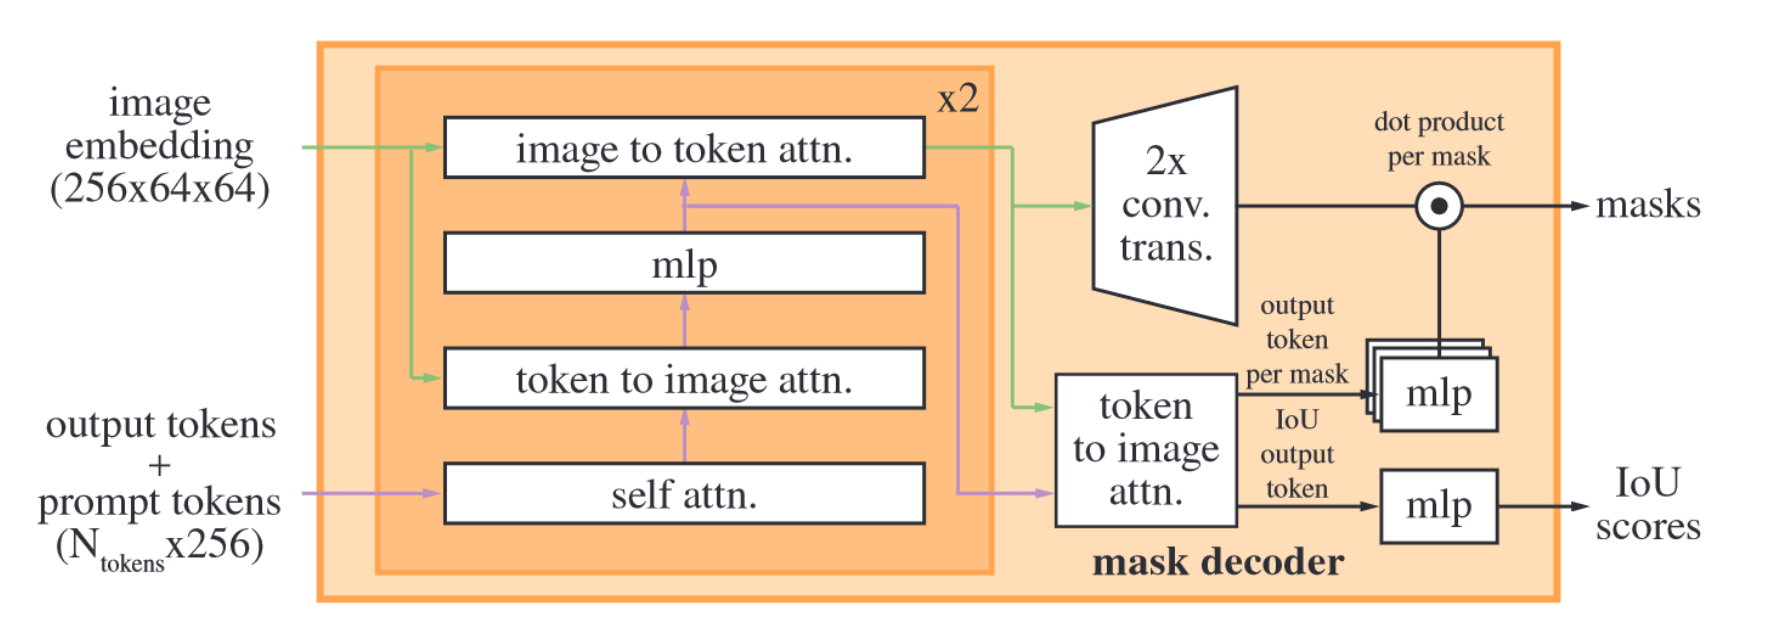
\includegraphics[width=0.6\textwidth]{img/segment-anything-model-mask-decoder.png}
  \vspace{0.25cm}
  \caption[The lightweight mask decoder design]{The lightweight mask decoder design \cite{kirillov2023segment}}
  \label{figure:segment-anything-model-mask-decoder}
\end{figure}

\begin{figure}[H]
  \centering
  \begin{subfigure}[b]{0.48\textwidth}
    \centering
    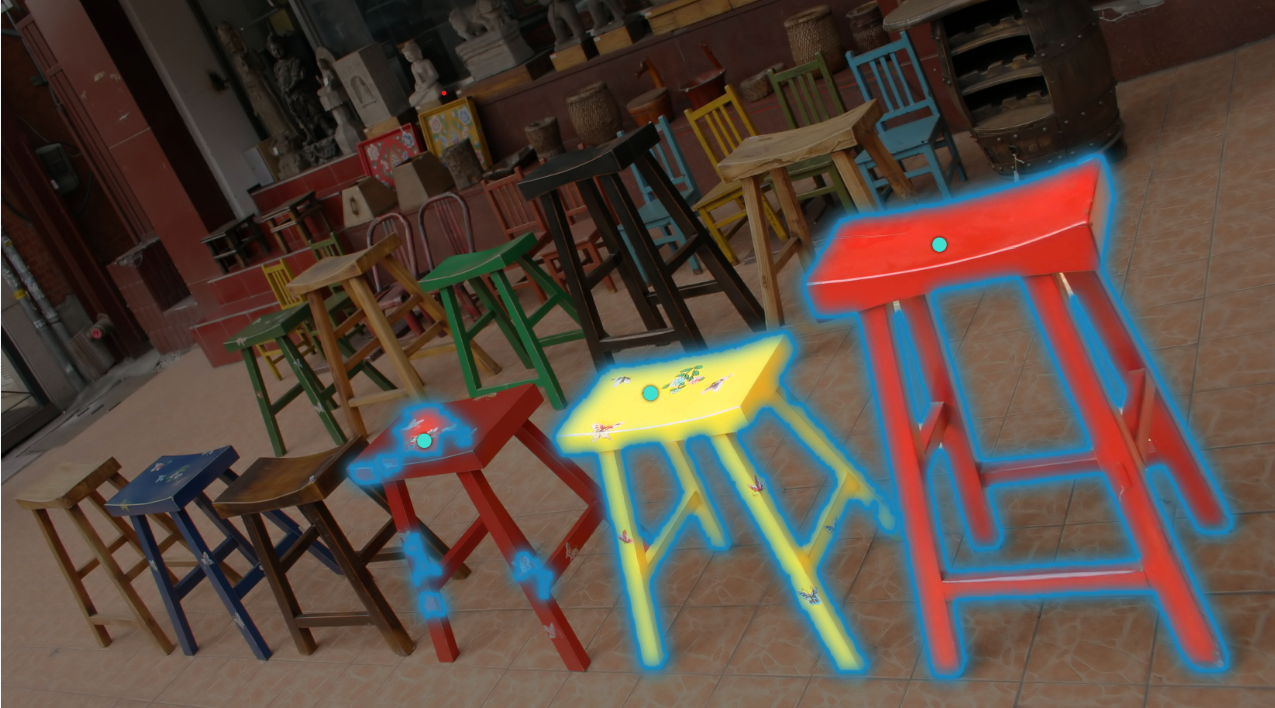
\includegraphics[width=\textwidth]{img/sam-segmented-after-point.png}
    \label{fig:sam_point}
  \end{subfigure}
  \hfill
  \begin{subfigure}[b]{0.48\textwidth}
    \centering
    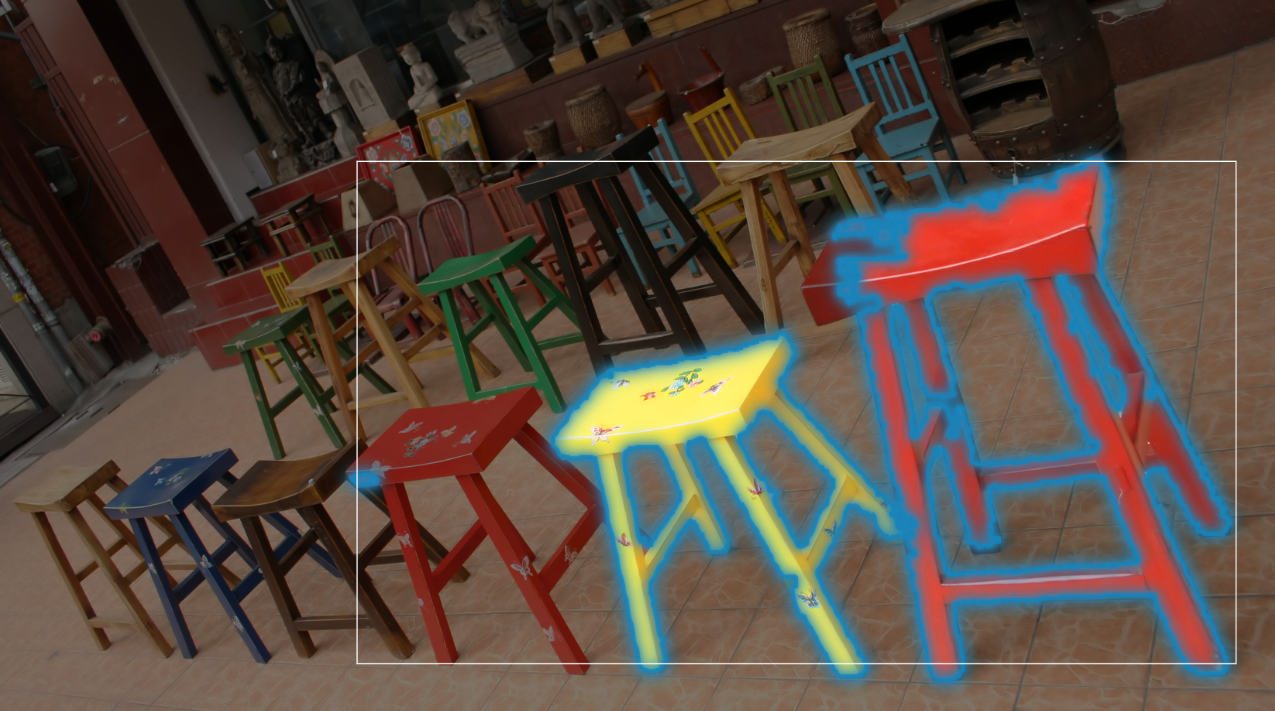
\includegraphics[width=\textwidth]{img/sam-segment-bounding-box.png}
    \label{fig:sam_box}
  \end{subfigure}
  \caption[Segmented regions returned by SAM]{Segmented regions returned by SAM. In the left figure, three points are selected, while in the right figure, a box is drawn. In both cases, the leftmost chair is not fully recognized.}
  \label{fig:sam_segments}
\end{figure}

\subsection{Image-to-Image Schrödinger Bridge}
\label{sec:i2sb}
Image inpainting is the process of restoring or completing portions of an image, the second phase in our watermark removal pipeline. After identifying the specific watermark location, image inpainting techniques can also be used to remove the visible watermarks \cite{huang2004attacking}. Thus, attention-guided inpainting methods, such as Partial Convolution \cite{liu2018image}, Contextual Attention \cite{yu2018generative} and Gated Convolution \cite{Yu:2018uw} are applicable to this task. Recently, Generative Adversarial Networks (GAN) \cite{goodfellow2014generative} and Image-to-Image Schrödinger Bridge (I$^2$SB) \cite{liu2023i2sb} are developed as state-of-the-art works. GAN trains two adversarial networks. A generator $G$ generates a sample $X$ as close to the dataset as possible and a discriminator $D$ labels the probability that $X$ is generated by $G$, not from the real dataset. Through adversarial training, $G$ and $D$ converge to the Nash equilibrium. On the other hand, I$^2$SB is developed recently from conditional diffusion models, using a tractable class of Schrödinger Bridge. As diffusion models are shown to beat GAN on image generation tasks \cite{dhariwal2021diffusion}, we present I$^2$SB as the main approach to our image inpainting task.

\begin{figure}[t]
  \begin{center}
    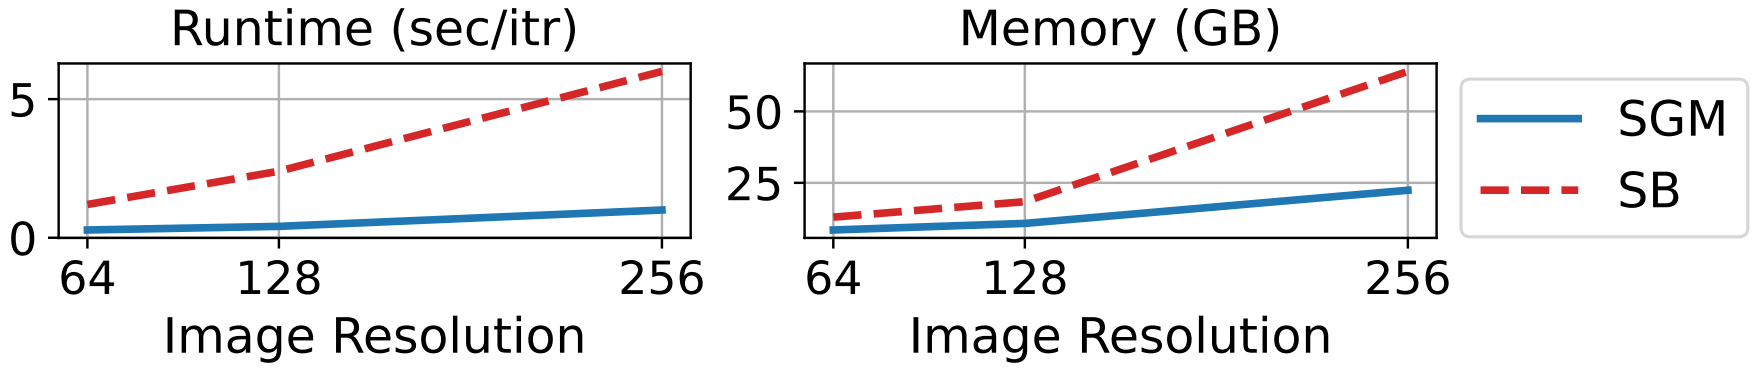
\includegraphics[width=0.85\columnwidth]{img/complexity.png}
    \caption[Complexity of SGM and SB]{
      Complexity of SGM and SB \cite{chen2021likelihood} On 256$\times$256 resolution, SB is 6$\times$ slower and consumes 3$\times$ memory.
    }
    \label{figure:complexity}
  \end{center}
\end{figure}

\begin{figure}[t]
    \centering
    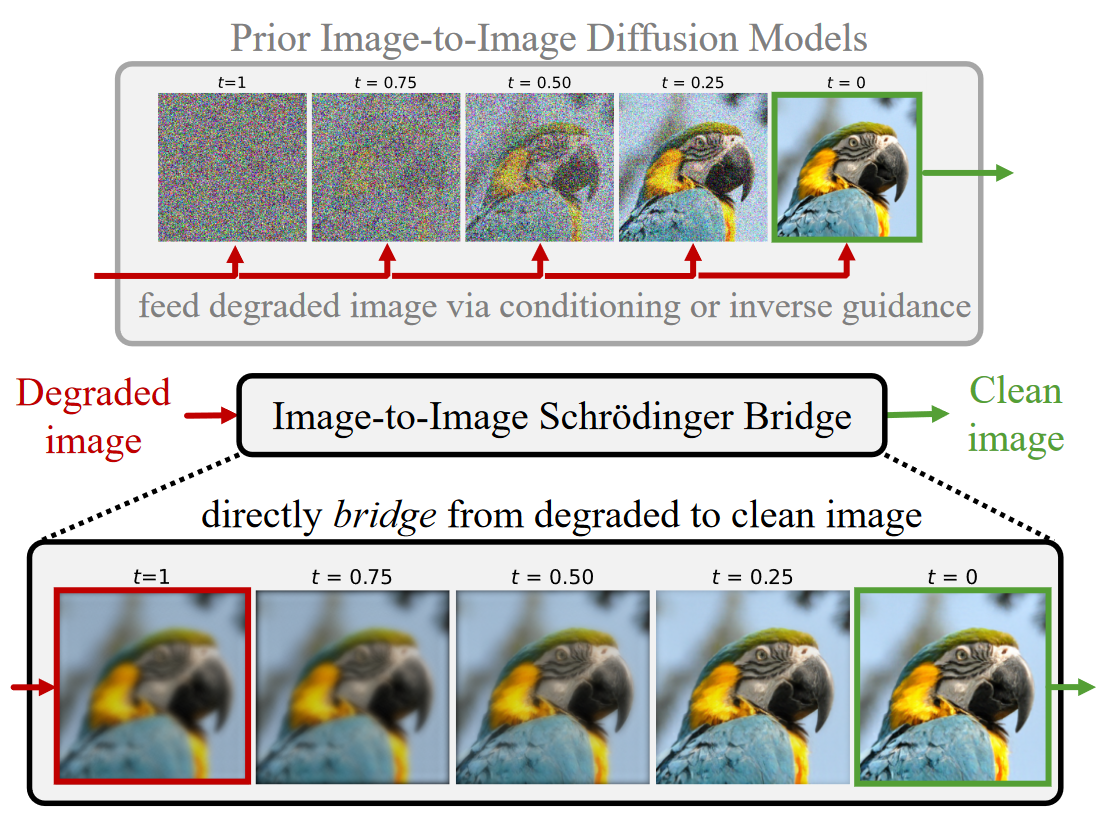
\includegraphics[width=0.6\linewidth]{diffusion-vs-sb.png}
    \caption{Difference between predominant non-conditional diffusion models and I$^2$SB}
    \label{figure:diffusion-vs-sb}
\end{figure}

Figure \ref{figure:complexity} illustrates the complexity of Likelihood Training of Schrödinger Bridge \cite{chen2021likelihood}, a previous SB approach (see Section \ref{section:diffusion-models}) for image generation. I$^2$SB employs a tractable class of SB for better training efficiency, cognizing that the train dataset is Dirac Delta distributed. The difference between non-conditional diffusion models and I$^2$SB can be seen in Figure \ref{figure:diffusion-vs-sb}. Non-conditional models generates a new sample in the image dataset distribution from the Gaussian noise, while I$^2$SB convert an image in the degraded distribution to an image in the clear distribution. 

\begin{sbtheorem}[Tractable SB with the Dirac Delta Boundary]
  \label{theo-dirac}
  Let $p(\cdot,0) := \delta_a(\cdot)$ be the Dirac delta distribution centered at $a\in\RR^d$. Then, the initial distributions in (\ref{equation:sde-psihat}) and (\ref{equation:sde-psi}) are given by
  \begin{equation}
    \label{equation:sb-dirac}
    \hat{\Psi}(\cdot,0)= \delta_A(\cdot), \Psi(\cdot,1)=\dfrac{p(\cdot, 1)}{\hat{\Psi}(\cdot,1)}.
  \end{equation}
\end{sbtheorem}

The Dirac delta assumption also implicitly appears in the denoising objective, which first computes the target $\nabla\log p(\xbf_t,t|\xbf_0=a)$ for each data point $a$, as the score between $\delta_{a}(\cdot)$ and Gaussian, then averages over $\xbf_0 {\sim} p_\A$. In this vein, Theorem \ref{theo-dirac} adopts the same boundary $\delta_{a}(\cdot)$ on one side and generalizes the other side from Gaussian to arbitrary $p_\B$. Based on the details provided in Table \ref{table:comp_diff}, it becomes evident that employing Theorem \ref{theo-dirac} enables us to transform the Schrödinger Bridge (SB) model, which is challenging to handle at $\nabla\log\hat{\psi}$ and demands substantial time and resources for training. With our model I$^2$SB, utilizing the degraded dataset allows us to generate a pair of information from the clean image. Consequently, the term $\nabla\log\hat{\psi}$ becomes manageable, enabling us to calculate the score with reduced resource requirements.


\begin{table}[H]
  \caption[Comparison of different diffusion models in boundary distributions and tractability]{
    Comparison of different diffusion models in boundary distributions and tractability of forward and backward drifts. Note that I$^2$SB requires paired information compared to standard SB}
  \label{table:comp_diff}
  \label{table:comp}
  \vskip 0.05in
  \begin{center}
    \begin{small}
      \begin{tabular}{rclcc}
        \toprule
        \textbf{Model} & \textbf{$\mathbf{p(\xbf_0)}$} & \textbf{$\mathbf{p(\xbf_1)}$} & \textbf{$\mathbf{\gradlog \Psi}$} & \textbf{$\mathbf{\gradlog \Psihat}$} \\ [0.5ex]
        \midrule
        (C)SGM
                       & $p_\A$                        & $\N(0,I)$                     & 0                                 & tractable                            \\[0.5ex]
        \textbf{I$^2$SB}
                       & $p_\A$                        & $p_\B(\cdot|\xbf_0)$          & intractable                       & tractable                            \\[0.5ex]
        SB
                       & $p_\A$                        & $p_\B(\cdot)$                 & intractable                       & intractable                          \\
        \bottomrule
      \end{tabular}
    \end{small}
  \end{center}
  \vskip -0.15in
\end{table}

